\section{予備実験}
\label{sec:experiment}

\subsection{検証仮説と実験設計}

\ref{sec:method}節の仮説，すなわち
``残差予測によってILCの収束を満たすための性質が強まる'' ことを実験的に検証する．
評価には図\,\ref{fig:pick_and_place} に示す積み木のピックアンドプレースタスクを用い，
プレース位置の変位 $\bm{c} = [\mathit{c}_x,\, \mathit{c}_y]$（各軸方向への移動量，単位 mm）をラベルとして与えたとき，
実際のプレース変位がラベルに対してどのように変化するかを定量的に検証した．

\begin{figure}[t]
  \centering
  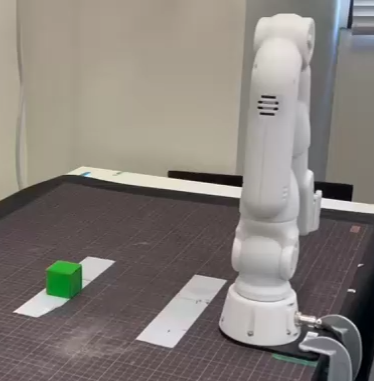
\includegraphics[width=0.92\linewidth]{figures/ExperimentEnvironment.png}
  \caption{ピックアンドプレースタスクの環境}
  \label{fig:pick_and_place}
\end{figure}

\subsection{学習データの収集}

まず，``掴んだ積み木をそのまま置く'' 基準動作をベース動作データとして収録した．
次に Motion Retouch を用いて，プレース位置を $X$・$Y$ 方向にそれぞれ $\pm5\,\text{mm}$ ずらした 8 箇所と，何も修正しなかった場合の 1 箇所，計 9 箇所に対して各 5 回の修正動作を収録し，合計 45 本のデータを収集した．
各修正動作にラベル $\bm{c} = [\mathit{c}_x, \mathit{c}_y]$ を付与し，
ベース動作データとの差分 $\Delta\xi^{(\bm{c})}$ を教師残差とした．

\subsection{検証モデル}

\begin{table*}[t]
  \centering
  \caption{検証モデルの一覧}
  \label{tab:models}
  \small
  \begin{tabular}{llll}
    \hline
    モデル名 & 入力 & 出力 & 特徴 \\
    \hline
    \texttt{Direct w/ image} & 関節状態・画像・ラベル & 絶対値（修正後） & 全ステップをNN予測 \\
    \texttt{Residual w/ image} & 関節状態・画像・ラベル & 残差 $\Delta\xi$ & ベース再生＋残差加算 \\
    \texttt{Residual w/o image} & 関節状態・ラベル & 残差 $\Delta\xi$ & 画像入力なし \\
    \hline
  \end{tabular}
\end{table*}

表\,\ref{tab:models} に示す 3 モデルを比較した．
\texttt{Direct w/ image} はロボットの観測とラベルから修正後動作データを直接予測する．
\texttt{Residual w/ image} と \texttt{Residual w/o image} は残差 $\Delta\xi$ を予測し，
実行時はモーションコピーで再生したベース動作データに残差を加算することで動作を生成する．
モーションコピーとは，ベース動作データから得られた関節角指令値をそのままロボットに入力して動作を再現するシステムであり，本研究ではラベル $\bm{c} = [0,0]$ の補正なしに対応する動作の基準として機能する．
ハードウェア再現精度の上限を確認するため，モーションコピー単体（\texttt{Motion Copy}）の計測値も評価基準として用いた．

\subsection{評価方法と試行数}

検証ラベルは，各成分が $\{-7, -5, -3, 0, 3, 5, 7\}$ の 7 値をとる 2 次元格子のうち，
原点・各座標軸・対角線上に配置した 25 種類とした．
把持動作が成立しない組み合わせはモデルごとに除外している
（\texttt{Direct w/ image}：4 ラベル除外，105 試行；\texttt{Residual w/o image}：2 ラベル除外，115 試行；\texttt{Residual w/ image}：全ラベル実施，125 試行）．

評価指標として以下を用いた：
\begin{itemize}
  \item ラベルと実変位の決定係数 $R^2$ および Spearman 順位相関係数 $\rho$（単調増加性の指標）
  \item ラベル $\bm{c} = [0,0]$ 時のプレース位置オフセット（残差ゼロの再現精度）
  \item 同一ラベル内の試行間標準偏差 $\sigma$（再現性）
  \item プレース・ピック時の手先姿勢偏差
\end{itemize}
